	\documentclass[10pt,oneside]{CBFT_book}
	% Algunos paquetes
	\usepackage{amssymb}
	\usepackage{amsmath}
	\usepackage{graphicx}
% 	\usepackage{libertine}
% 	\usepackage[bold-style=TeX]{unicode-math}
	\usepackage{lipsum}

	\usepackage{natbib}
	\setcitestyle{square}

	\usepackage{polyglossia}
	\setdefaultlanguage{spanish}
	



	\usepackage{CBFT.estilo} % Cargo la hoja de estilo

	% Tipografías
	% \setromanfont[Mapping=tex-text]{Linux Libertine O}
	% \setsansfont[Mapping=tex-text]{DejaVu Sans}
	% \setmonofont[Mapping=tex-text]{DejaVu Sans Mono}

	%===================================================================
	%	DOCUMENTO PROPIAMENTE DICHO
	%===================================================================

\begin{document}

% =================================================================================================
\chapter{Introducción al estudio de procesos de relajación}
% =================================================================================================


% =================================================================================================
\section{Procesos de Markov}
% =================================================================================================

Sea $Y$ una variable estocástica (aquellas que provienen de experimentos, donde no se tiene información
dinámica determinista\footnote{No tengo información para predecir nada.}) 
que puede tomar valores $y_1, y_2,...$\notamargen{Las $P$ son densidades
de probabilidad, cuando el espacio muestral sea continuo.}
\[
	P_1(y_1,t) \equiv \text{Prob. de tomar $y_1$ en tiempo $t$ (1 paso)}
\]
\[
	P_2(y_1,t_1;y_2,t_2) \equiv \text{Prob. de tomar $y_1$ en $t_1$ y $y_2$ en $t_2$ (conjunta)}
\]
Para $N$ pasos es
\[
	P_N(y_1,t_1;y_2,t_2; ...; y_N,t_N) 
\]
\[
	P_{1/1}(y_1,t_1 | y_2, t_2) \equiv \text{Prob. condicional de tomar $y_2$ en $t_2$ habiendo 
	tomado $y_1$ en $t_1$ (certeza de $y_1$) }
\]
\notamargen{Es importante que la condicional implica que se sabe algo con certeza.}

Abreviaremos obviando el tiempo. Además se tiene 
\[
	P(y_1;y_2) \leq P(y_1 | y_2)
\]
donde el lhs evalúa los caminos que comunican $y_1, y_2$ del total y el rhs evalúa los cminos que comunican
$y_1, y_2$ del subconjunto de los que parten de $y_1$.

Además
\[
	P_2(y_1;y_2) = P_1(y_1) P_{1/1}(y_1|y_2),
\]
que es el caso de $P(B)P(B/A)=P(A)$, cumpliéndose lo siguiente
\begin{itemize}
	\item $ \int P_1(y_1) dy_1 = 1 \qquad  \text{normalización} $ 
	\item $ \int P_{1/1}(y_1|y_2) dy_2 = 1 \qquad \text{normalización} $ 
	\item $ \int P_2(y_1;y_2) dy_1 = \int P_1(y_1) P_{1/1}(y_1|y_2) dy_1 =  P_1(y_2) 
	\qquad \text{reducción} $
\end{itemize}
La integral de normalización implica sumar todos los caminos de $(y_1,t_1)$ a $(y_2,t_2)$.

La reducción se puede definir en general para $N$ pasos y $N-1$.
Cuando la densidad de probabilidad es invariante ante una traslación temporal se dice que es estacionaria.
En ese caso se da que
\[
	P_N(y_1,t_1;y_2,t_2; ...; y_N,t_N) = P_N(y_1,t_1+\tau;y_2,t_2+\tau; ...; y_N,t_N+\tau) 
\]

\subsubsection{Ejemplito numérico}

\[
	P(y_1;y_2) = P(y_1)P(y_1|y_2) = \frac{4}{4}\frac{1}{2} = \frac{2}{7}
\]
\[
	P(y_2;y_1) = P(y_2)P(y_2|y_1)  = \frac{3}{7}\frac{2}{3} = \frac{2}{7}
\]
Notemos que $P(A|B) \neq P(B|A)$ aunque $P(A;B) = P(B;A)$

Las densidades de muchos pasos: $P(y_1;y_2;y_3)$ son relevantes cuando el sistema tiene ``memoria''.
Se clasifican los procesos en función de la memoria; en el caso de Markov nos preocupamos del último
anerior y requeriré la probabilidad de un evento y la probabilidad de transición: estas dos cosas
definen los procesos de Markov.

Un proceso es de Markov cuando el estado del sistema depende del paso inmediato anterior únicamente.
Se define por 
\[
	P_1(y_1) , \quad P_{1/1}(y_1|y_2) \equiv \text{Probabilidad de transición} 
\]
\[
	P_{3/1}(y_1,y_2,y_3|y_4) \underbrace{\rightarrow}_{\text{Markov}} \; P_{1/1}(y_3|y_4)
\]
luego, conociendo
\[
	\begin{cases}
	P_1 ( y, t )  \\
	P_{1/1}( y_{n-1}, t_{n-1} | y_n t_n )
	\end{cases}
\]
ya conozco todo lo que necesito.


Se puede demostrar una ecuación de Chapman-Kolmogorov
\[
	P_{1/1}(y_1|y_3) = \int P_{1/1}(y_1|y_2) P_{1/1}(y_2|y_3) dy_2
\]
que se interpreta como la suma en todos los caminos. Se tiene el constraint de que la norma debe
conservarse en el tiempo.

% ~~~~~~~~~~~~~~~~~~~~~~~~~~~~~~~~~~~~~~~~~~~~~~~~~~~~~~~~~~~~~~~
\subsection{Ecuación maestra}

Queremos ver la evolución de la $P_1(y_1,t)$
\[
	\dtot{P_1(y,t)}{t} = \lim_{\tau \to 0} \frac{P_1(y,t+\tau) - P_1(y,t) }{\tau}
\]
Usando que
\[
	P_1(y_2,t+\tau) = \int dy_1 P_1(y_1,t) P_{1/1}(y_1,t|y_2,t+\tau) 
\]
\[
	P_1(y_2,t) = \int dy_1 P_1(y_1,t) P_{1/1}(y_1,t|y_2,t) 
\]
\[
	\dtot{P_1(y,t)}{t} = \int dy_1 P_1(y_1,t) \left[ \lim_{\tau \to 0} 
	\frac{1}{\tau} (P_{1/1}(y_1,t|y_2,t+\tau) - P_{1/1}(y_1,t|y_2,t))   \right]
\]
que se puede escribir de modo que 
\[
	\frac{1}{\tau} \left\{ [ 1 - \tau \int dy W(y_1,y)]\delta(y_1 - y_2) + 
	\tau W(y_1,y_2) - \delta(y_1-y_2) \right\}
\]
y entonces 
\[
	\dtot{P_1(y,t)}{t} = \int dy_1 P_1(y_1,t) 
	\left[ -\int dy W(y_1,y) \delta(y_1-y_2) + W(y_1,y_2) \right]
\]
\[
	\dtot{P_1(y,t)}{t} = \int dy_1 P_1(y_1,t) W(y_1,y_2) - \int dy_1 P_1(y_1,t) \int dy W(y_1,y)\delta(y_1-y_2)
\]
\[
	\dtot{P_1(y,t)}{t} = \int dy_1 P_1(y_1,t) W(y_1,y_2) - \int dy P_1(y_2,t) W(y_2,y)
\]
\[
	\dtot{P_1(y,t)}{t} = \int dy_1 P_1(y_1,t) W(y_1,y_2) - P_1(y_2,t) \int dy  W(y_2,y)
\]
donde el primer término en el rhs se interpreta como ganancia (lo que entra) y el segundo la
pérdida (pues la integral es lo que sale).
\[
	W(y_1,y_2) \equiv \text{Transiciones $y_1\to y_2$ por la unidad de tiempo}
\]

Si la densidad de probabilidad es nula puede ser que haya un balance entre lo IN y OUT.
Equilibrio no significa necesariamente que no pase nada; puede ser ese balance.


\begin{center}
	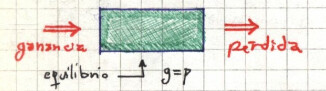
\includegraphics[scale=0.5]{images/1606329165.jpg}
	% asfdasdf.: 0x0 pixel, 0dpi, 0.00x0.00 cm, bb=
\end{center}


% ~~~~~~~~~~~~~~~~~~~~~~~~~~~~~~~~~~~~~~~~~~~~~~~~~~~~~~~~~~~~~~~
\subsection{Camino aleatorio y ecuación de difusión}

Si $\ell, \Tau$ son escalas y $n_2,s$ un número entero de pasos 
\[
	P_1(n_2\ell, s\Tau ) = 
	\sum_{n_1} P_1( n_1\ell, [s-1]\Tau )P_{1/1}( n_1\ell, [s-1]\Tau|n_2\ell, s\Tau )
\]
Quiero saber cuáles son las chances de estar en $n_2\ell$ al tiempo $s\Tau$ sumando todas 
las transiciones desde diferentes lugares $n_1\ell$.

Si la probabilidad es uniforme 
\[
	P_{1/1}(n_1\ell,[s-1]\Tau|n_2\ell,s\Tau) =
	\frac{1}{2}\delta(n_2-[n_1+1]) + \frac{1}{2}\delta(n_2-[n_1-1]) = \frac{1}{2}
	\begin{cases}
	 \text{si} \; n_2 = n_1 + 1 \\
	 \text{si} \; n_2 = n_1 - 1
	\end{cases}
\]
\[
	P_1(n_2\ell,s\Tau) = \sum_{n_1} P_1(n_1\ell,[s-1]\Tau)\left\{
	\frac{1}{2}\delta(n_2-[n_1+1]) + \frac{1}{2}\delta(n_2-[n_1-1])
	\right\}
\]
y sumando y restando convenientemente,
\[
	P_1(n_2\ell,s\Tau) = -\frac{1}{2}P_1([n_2-1]\ell,[s-1]\Tau) + 
\frac{1}{2}P_1([n_2+1]\ell,[s-1]\Tau)
	+ P_1(n_2\ell,[s-1]\Tau) - P_1(n_2\ell,[s-1]\Tau)
\]
\begin{multline}
	\frac{P_1(n_2\ell,s\Tau) - P_1(n_2\ell,s\Tau)}{\Tau} = \\
	\frac{\ell^2}{2\Tau} \left[ \frac{ P_1([n_2-1]\ell,[s-1]\Tau) - 
2P_1(n_2\ell,[s-1]\Tau) + P_1([n_2+1]\ell,[s-1]\Tau) }{\ell^2} \right] 
\end{multline}


Pero esto no es otra cosa que expresiones de las derivadas, de manera que
\[
	\frac{\delta P(n_2\ell,s\Tau)}{\delta \Tau} =
	\frac{\ell^2}{2\Tau} \frac{\delta^2 P(n_2\ell,[s-1]\Tau)}{\delta\ell^2}
\]

Esta es la ecuación de Fokker-Planck
\[
	\dpar{P(x,t)}{t} = C \dpar[2]{P(x,t)}{x}
\]
una ecuación de onda para la probabilidad (?)


\section{Cadenas de Markov}

Espacio muestral discreto $Y=\{ y_1, y_2, y_3,...,y_\ell \}$ de dimensión $L$ y donde
medimos el tiempo en pasos.
Se tiene una ecuación de evolución dada por
\[
	P_1(y_j,s+1) = \sum_i^L P_1(y_i,s) P_{1/1}(y_i,s|y_j,s+1),
\]
que es la probabilidad de llegar a un estado específico desde todos los otros posibles y
donde la información sobre las transiciones se introduce en la matriz $Q$ tal que 
\[
	Q_{ij} \equiv P_{1/1}(y_i,0|y_j,1),
\]
que es la matriz estocástica.
Se verifica
\[
	\sum_i^L Q_{ij} = 1 \; \forall i
\]
y entonces las filas son vectores de probabilidad\footnote{Tenía anotado que si
la suma de las filas es 1 entonces la matriz se llama estocástica}
\[
	\overbrace{\vec{P(1)}}^{1\times L} =  \overbrace{\vec{P(0)}}^{1\times L} 
\overbrace{Q}^{L\times L}
\]
\[
	P_j(1) = P_i(0) Q_{ij} \quad \text{Asumimos convención de Einstein}
\]
\notamargen{La matriz $Q$ tiene probabilidades de transición fijas en el tiempo,
de modo que $Q$ es independiente del tiempo.}
\[
	\vec{P(s)} = \vec{P(s-1)}Q = \vec{P(s-2)} Q Q = ... = \vec{P(0)}Q^s
\] 
y decimos que $Q$ es estocástica regular si existe $k : [Q^k]_{ij} > 0 \forall i,j$.


Si $Q$ es estocástica regular entonces existe $s : Q^{s+1} = Q^s \equiv T$ y por lo tanto
\[
	Q T = Q^{s+1} = T
\]
\notamargen{$T$ es la solución de equilibrio, pues $T=QT$}
Si $n>s$
\[
	\vec{P(n)} = \vec{P(0)} Q^n = \vec{P(0)} Q^{n-s} Q^s = \vec{P(0)} T
\]

\[
	\lambda_\alpha \overbrace{\vec{P}^\alpha}^{1\times L} =  
	\overbrace{\vec{P}^\alpha}^{1\times L} \overbrace{Q}^{L\times L}
	\quad \rightarrow \quad 0 = \vec{P}^\alpha (Q-\lambda_\alpha \mathbb{1}) 
\]
\[
	\lambda_\beta \overbrace{\vec{P}^\beta}^{1\times L} = 
	\overbrace{\vec{P}^\beta}^{1\times L} \overbrace{Q}^{L\times L}
	\quad \rightarrow \quad  0 = (Q-\lambda_\beta \mathbb{1}) \vec{P}^\beta
\]
y tenemos autovalores a izquierda
\[
	\lambda_\alpha \chi_j^\alpha = \chi_{1i}^\alpha Q_{ij} \qquad \vec{\chi} = (,,,)
\]
donde los índices $j,1i$ refieren a columnas y autovalores a derecha
\[
	\lambda_\beta \psi_{i1}^\beta = Q_{ij} \psi_{j1}^\beta \qquad \vec{\chi} = 
									\begin{pmatrix}
									\\
                                                                        \\
                                                                        
                                                                        \end{pmatrix}
\]
donde los índices $i1,j1$ refieren a filas.
Parece que el hecho de que $Q$ sea no simétrica impalica que tiene autovalores a izquierda
y derecha.


Y entonces deducimos que 
\begin{itemize}
 \item Autovectores a izquierda $\vec{\chi}$ y a derecha $\vec{\psi}$ son ortogonales.
 \item Los autovalores son $|\lambda_\gamma|\leq 1$.
 \item $\lambda = 1$ es siempre autovalor.
\end{itemize}

Sabemos que 
\[
	P(m,s) = \sum_n P(n,0) Q^s_{nm},
\]
\notamargen{En algún momento tuvimos que decir que esto es sumar sobre todos los caminos de
llegar al punto final.}
y con $s=1$
\[
	P(m,1) = \sum_n P(n,0) Q_{nm}
\]
y esto es 
\[
	\chi_m = \sum_n \chi_n Q_{nm}  \qquad (\lambda=1 \text{autovalor de $\vec{\chi}$ 
estacionario})
\]
\notamargen{Siempre hay solución estacionaria $P=PQ$.}

Para el autovector a derecha 
\[
	\lambda_\beta \psi_{\ell 1}^\beta = \sum_i Q_{\ell i} \psi_{i1}^\beta
\]

Si $ \vec{\psi}^\beta = (1,1,...,1)^t\rightarrow$
\[
	\lambda_\beta \psi_\ell^\beta = \lambda_\beta = \sum_i Q_{\ell i} \psi_i^\beta
	= \sum_i Q_{\ell i} = 1
\]
y $\lambda_\beta=1$ autovalor de 
\[
	\vec{\psi}^\beta = \begin{pmatrix}
	 1\\
	 1\\
	 ...\\
	 1
	\end{pmatrix}
\]

\subsection{Solución general a través de descomposición espectral}

\[
	\lambda_\alpha \chi_i^\alpha = \sum_j \chi_j^\alpha Q_{ij} 
\]
\[
	\lambda_\alpha \psi_\ell^\alpha \chi_i^\alpha = \sum_j \psi_\ell^\alpha\chi_j^\alpha Q_{ij} 
\]
\[
	\sum_\alpha \lambda_\alpha \psi_\ell^\alpha \chi_i^\alpha = 
	\sum_j \sum_\alpha \psi_\ell^\alpha\chi_j^\alpha Q_{ij} =
	\sum_j \delta_{\ell j} Q_{ji} = Q_{\ell i}
\]
y entonces 
\[
	Q_{\ell i} = \sum_\alpha \lambda_\alpha \psi_\ell^\alpha \chi_i^\alpha
\]
es una descomposición espectral, análoga a la de mecánica cuántica $\mathbb{1} = \sum_i \Ket{i}\Bra{i}$.
Esto sería la clausura, que sume uno. Y la completitud ortogonalidad sería $\chi_i \psi_j = \delta_{ij}$.
De esta forma 
\[
	Q_{\ell i}^s = \sum_\alpha \lambda_\alpha^s \psi_\ell^\alpha \chi_i^\alpha
\]
por ortogonalidad de $( \vec{\chi}, \vec{\psi} )$.

\[
	Q_{\ell i}^s = \lambda_1^s \psi_\ell^1 \chi_i^1 + 
	\sum_{\alpha=2} \lambda_\alpha^s \psi_\ell^\alpha \chi_i^\alpha
\]
Y si $s \to \infty$ entonces $\lambda_1 = 1$ y $\psi^1 = (1,1,...,1)^t$, mientras que
$\lambda^s_{\a}$ tiende a cero puesto que $ |\lambda_i| \leq 1$, de modo que 
\[
	\lim_{s\to \infty} Q^s_{\ell i} = \overbrace{\psi_\ell^1}^{L\times 1} 
	\overbrace{\chi_\ell^1}^{L\times 1} = \begin{bmatrix}
	                                       \begin{pmatrix}
	                                        1 \\
	                                        1 \\ 
	                                        ... \\
	                                        1
	                                       \end{pmatrix}
						(\chi_1^1 \chi_2^1 ... \chi_L^1 )
	                                      \end{bmatrix}_{\ell i}
	= \chi_i^1
\]
\notamargen{Todas las filas son iguales.}
\[
	\lim_{s\to \infty} Q^s_{\ell i} = T_{\ell i} = \chi_i^1 \quad \forall \ell
\]
entonces
\[
	T = \begin{pmatrix}
	     [ \; \chi^1 \ ; ] \\
	     [ \; \chi^1 \ ; ] \\
	     ...\\
	     [ \; \chi^1 \ ; ]
	    \end{pmatrix}
\]

Luego $T$ tiene como filas al autovector que cumple
\[
	\vec{\chi} = \vec{\chi} Q \qquad \text{El punto fijo de $Q$}
\]
Por otro lado
\[
	\lim_{s\to \infty} Q^s_{\ell i} = \lim_{s\to \infty} P_{1/1}(\ell, 0 | i,s) = P_1(i,0)
\]

La probabilidad de un estado $i$ final, una vez dentro del régimen estacionario, no depende del estado
$\ell$ desde el cual partimos.
Tenía anotado algo como que haciendo el límite $s \to \infty$ se puede escribir
\[
	P(n,s) = \sum_{m=1}^N \: P(m,0) \psi_1(n) = \psi_1(n)
\]
y el $\psi_1(n)$ no depende desde donde partí (luego de muchos pasos) y entonces el autovector que
podemos interpretar como probabilidad es el $\psi_1(n)$ porque está asociado a que es una
tendencia asintótica.

La solución de equilibrio claramente es
\[
	\vec{P} = \vec{P} Q 
\]
pues si $\vec{P}(s+1) = \vec{P}(s)Q$ y obtenemos
\[
	\vec{P}(s+1) = \vec{P}(s) = \vec{P}(s)Q
\]
entonces resulta que 
\[
	\vec{P}(s)  = \vec{P}(s) Q
\]
es lo que hay que buscar.
La moraleja es que $\vec{P}$ de equilibrio es el punto fijo de $Q$.

\notamargen{Los siguientes problemas aparecían en la página 14 de la carpeta, tal vez correspondan
a algún capítulo inicial más que aquí.}

\begin{ejemplo}{\bf Problema 4}
 
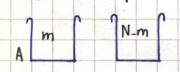
\includegraphics[width=0.30\textwidth]{images/1606329215.jpg}

Se elige una bocha, y se cambia de urna. Las bochas se eligen completamente al azar; no sé de qué 
tarro las voy a tomar.
La idea es que evolucionamos de $n' \to n$, entonces
\[
	T_{nn' } = \frac{n}{N} \delta_{n+1,n'} + \left[ 1 - \frac{n'}{N} \right] \delta_{n-1,n'}
\]
que interpreta al primer término como el vaciamiento de A y al segundo como el llenado de A.

Definiendo $y \equiv N_A$ queremos ver las psobiels transiciones

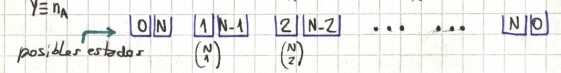
\includegraphics[width=0.90\textwidth]{images/1610808616.jpg}

No me precoupan las diferentes combinaciones de cada estado. No pienso en variaciones microscópicas.
\[
	T_{10} = 1 \qquad \qquad T_{01} = \frac 1 N \qquad \qquad 
	T_{21} = \frac {N-1} N \qquad \qquad T_{12} = \frac 2 N
\]
Entonces,
\[
	P(n,s+1) = \sum_{m=0}^N \: P(m,0) Q_{mn}^s = \sum_{m=0}^N \: P(m,s) Q_{mn}
\]
\[
	P(n,s+1) = \sum_{m=0}^N \: P(m,s) 
	\left( \frac{m}{N} \delta_{n,m-1} + \left[ 1 - \frac{m}{N} \right] \delta_{n,m+1} \right)
\]
\[
	P(n,s+1) = \frac{n+1}{N} P(n+1,s) + \left[ 1 - \frac{n-1}{N} \right] P(n-1,s)
\]
para $1 \leq n \leq n-1$. Como $P(0,s+1) = 1/N P(1,s)$ y $P(N,s+1)=1/N P(N-1,s)$ si tomamos esta
podemos ver que satisface la ecuación última.
A tiempos muy grandes esperaríamos $P(n)=(m/n) 1/2^N$ y se puede ver reemplazando y viendo que se
plancha la evolución temporal.
 
\end{ejemplo}

\begin{ejemplo}{\bf Problema 6}

Una bola de cada una y se intercambian

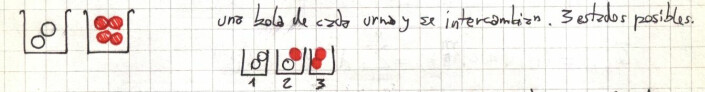
\includegraphics[width=0.90\textwidth]{images/1606329219.jpg}

La matriz de transición sería algo como
\[
	\begin{pmatrix}
	 0 	&	1	&	0	\\
	 1/8 	&	1/2	&	3/8	\\
	 0 	&	1/2	&	1/2	
	\end{pmatrix}
\]
y los autovalores $\lambda_i = 1, 1/4, -1/4$ para $i=1,2,3$.
Los autovalores a derecha
\[
	\psi_1 = (1,1,1) \qquad 
	\psi_1 = (2,-1/2,1) \qquad 
	\psi_1 = (1,-1/4,1/6) 
\]
y los autovalores a izquierda
\[
	\chi_1 = ( 1/15, 8/15, 6/15 ) \qquad
	\chi_2 = ( -1/2, -1, -3/2 ) \qquad 
	\chi_3 = ( 7/6, -4/6, -7/6 ) 
\]
Se tienen además
\[
	P^{(3)} = P(0) Q^3
\]
donde $Q^3$ será
\[
	Q^3 = \sum_{i=1}^3 \; \lambda_i^3  \psi_i \chi_i
\]
sujeta a las condiciones iniciales
\[
	P(0) = \begin{cases}
	 (1,0,0) \\
	 (0,0,1) \\
	 (0,1,0)
	\end{cases}.
\]

\notamargen{El sistema está en equilibrio cuando olvidó el punto desde el cual partió.}

\end{ejemplo}


\begin{ejemplo}{\bf Problema 7}

La picture ilustra el problema

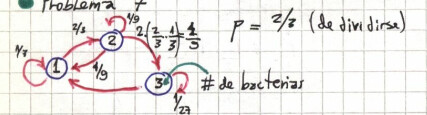
\includegraphics[scale=0.5]{images/1606329257.jpg}

que lleva a la matriz
\[
	Q = \begin{pmatrix}
		1/3 & 2/3 & 0 \\
		4/9 & 1/9 & 4/9 \\
		26/27 & 0 & 1/27 
	    \end{pmatrix}
\]
y los lugares que quedan nulos son de cosas que no están vinculadas.

Equilibrio significa que si llegarremos aun tiempo donde las probabilidades no dependen de
cuál fue el punto inicial. A ojo vemos que en un paso no se pueden conectar todos los
estados; pero en dos pasos sí se pueden conectar. Entonces existe $ \lambda = 1 $ tal que
\[
	\psi_1 = \begin{pmatrix}
	          1 \\
	          1 \\
	          1
	         \end{pmatrix}
	\qquad 
	\chi_1 = ( \: 52/109, 39/109, 18/109 \:)
\]
y es asintóticamente
\[
	P(n) = ( \: 52/109, 39/109, 18/109 \:)
\]
\[
	P(n_0,0) = (0,1,0)
\]
\[
	P(n,s=2) = \sum_{n_0=1}^3 \: P(n_0,0) Q_{n_0 n}^2 
\]

Si las bacterias mueren tengo que agregar un estado ``0'' absorbente: una vez que caigo no
puedo salir y entonces el estado asintótico será el de la muerte total (es nula la cantidad
de bacterias).
 
\end{ejemplo}

\begin{ejemplo}{\bf Problema 8}

Metemos el tiempo en lugar de la cantidad de pasos, entonces convertimos
\[
	P(n,s) \longrightarrow P(n,t)
\]
lo que dará origen a la ecuación maestras, donde $P(n,t)$ es claramente la probabilidad de estar en
un estado $n$ a tiempo $t$.
Tendremos
\be
	\dpar{P(n,t)}{t} = \sum_{m=1}^N \: 
	P(n,t) \omega_{mn}(t) - P(n,t) \omega_{nm}(t)
	maestra_prob_8
\ee
donde le primer término son las ganancias (probabilidad de estados que llegan a $n$) y el segundo las
pérdidas (probabilidad de estados que se van de $n$).

La $\omega_{mn}$ tendrá una forma que se modelará desde el sistema mismo. La función generatriz $F$
(que nos darán los distintos momentos de la distribución)
permite la resolución más sencilla de estos problemas.
\[
	F(z,t) = \sum_n \: P(n,t) z^n \qquad \qquad F(1,t)=1
\]
Desde 
\[
	\dpare{F}{z}{z=1} = \vm{n}_t
\]
obtengo los momentos por derivación.

Entonces se puede poner la caminata aleatoria simétrica

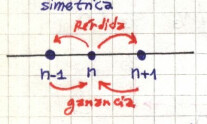
\includegraphics[scale=0.5]{images/1606329264.jpg}

como
\[
	\dot{p}_n = p_{n+1} + p_{n-1} - 2 p_n, \qquad -\infty < n < \infty 
\]
y se puede escribir la \eqref{maestra_prob_8} como una ecuación para $ \Gamma$
\[
	\dot{p}_n = \frac{1}{2} p_{n+1} + \frac{1}{2} p_{n-1} - p_n, \qquad -\infty < n < \infty 
\]
con el tiempo reescalado. Ahora necesito una ecuación para $F$,
\[
	\sum_{n=-\infty}^\infty \: z^n \dpar{P_n}{t} = 
	\sum_{n=-\infty}^\infty \: z^n p_{n+1} + z^n p_{n-1} - 2 z^n p_{n}
\]
luego
\[
	\dpar{F(z,t)}{t} = \sum_{n'} \frac{z^{n'}}{z} p_{n'} + 
	z^{n'} p_{n'} - 2 \: z^{n'} p_{n'}
\]
de lo cual finalmente resulta
\[
	\dpar{F(z,t)}{t} = \left[ \sum_n z^n p_n \right]\left( \frac{1}{z} + z - 2  \right)
	= F \frac{(z-1)^2}{z}
\]
donde el factor del final no depende del tiempo $t$. Entonces
\[
	F(z,t) = F(z,0) \euler^{ \frac{(z-1)^2}{z} t }
\]
y con $F(1,t)=1=F(z,0)$ se tiene $F(z,t) = \euler^{ \frac{(z-1)^2}{z} t }$.

Con esto salen los momentos derivando simplemente. Asimismo podemos identificar direcctaamnte
a mano
\[
	F(z,t) = \sum_n \: P(n,t) z^n
\]
donde los $P$ serán las probabilidades entregadas sin sacrificio al poner la exponencial en
términos de la serie.
 
\end{ejemplo}

\begin{ejemplo}{\bf Ejemplo ilustrativo de la práctica}

Consideramos una población de bacterias con las siguientes características
\[
	\text{Prob. de morir en } (t,t+dt) \qquad \omega_{n n-1}(t)\Delta t = d_n(t)\Delta t
\]
\[
	\text{Prob. de nacer en } (t,t+dt) \qquad \omega_{n n+1}(t)\Delta t = b_n(t)\Delta t
\]
\[
	\text{Prob. de que no ocurra nada en } (t,t+dt) \qquad ( 1 - [ b_{n}(t) + d_n (t) ] ) \Delta t 
\]

Además, consideraremos $\Delta t$ tan chico que no ocurren dos eventos simultáneos. Una sola
transición. La ecuación maestra implica ganancia y pérdida.
\[
	\dpar{P(n,t)}{t} = b_{n-1}(t) P(n-1,t) +
	d_{n+1}(t) P(n+1,t) - ( b_{n}(t) + d_{n}(t) ) P(n,t)
\]
Suponemos procesos lineales de nacimiento y muerte, que no dependen del tiempo.
\[
	b_n(t) = \beta n \qquad d_n(t) = \gamma n
\]
donde $\beta,\gamma$ son probabilidades por unidad de bacterias.
\[
	\dpar{P(n,t)}{t} = \beta (n-1) P(n-1,t) +
	\gamma (n+1) P(n+1,t) - (\beta n + \gamma n ) P(n,t)
\]
Si la ecuación anterior da $P(n=-1) \neq 0$ estamos ante un absurdo físico que deberá interpretarse.
En general debo poner un vínculo para respetar la física
\[
	F(z,t) = \sum_{n=-\infty}^\infty \: z^n P(n,t)
\]
que es que sumo desde menos infinito pero en realidad no aporta porque la ecuación está acotada 
naturalmente; $n=0$. No tengo manera de poblar estados con $n < 0$.
de la cual {\it amasando} podemos llegar a
\[
	\dpar{F(z,t)}{t} = (z-1)(\beta z - \gamma) \dpar{F(z,t)}{z}
\]
la cual a su vez puede resolverse por un método de las características.
\[
	\dpar{F(z,t)}{t} + g(z) \dpar{F(z,t)}{z} + h(z) F(z,t) = 0
\]

Con este tipo de ecuación podemos pensar en
\[
	F(z,t) = \euler^{-\int^t h(z)/g(z) dz} \phi( z, t),
\]
con lo cual llegamos a
\[
	\dpar{\phi(z,t)}{t} + g(z) \dpar{\phi(z,t)}{z} = 0 
	\qquad dt = \frac{dz}{g(z)}
\]
y genero las curfvas de niveles constantes de $ \phi $ de modo que $\phi$ será constante si me muevo
en $dz, dt= dz/g(z)$.
Entonces como se tiene
\[
	\int^z \frac{d(z')}{g(t)} - t = c_1
\]
esto nos conduce a 
\[
	\phi(z,t) = ºphi \euler^{ \frac{dz}{g(z)-t}}
\]
y
\[
	F(z,t) = \euler^{\int^t h(t)/g(z)} \phi( \euler^{\int^z dz/g(z) -t}).
\]
Volviendo al problema original, tendremos
\[
	F(z,t) = \Frac{ \beta(z-1) \euler^{(\beta - \gamma)t} }{\beta z - \gamma}^m
\]
Mediante condiciones iniciales puedo decir algo de $F$.
Si a $t=0$ hay $m$ bacterias entonces $P(m,0) = \delta_{nm}$
\[
	F\Frac{\beta(z-1)}{\beta z - \gamma} = z^m \quad \to \quad 
	F(\mu) = \Frac{\gamma \mu - \beta}{\beta(\mu -\beta)}^m
\]
donde hemos redefinido $\mu \equiv \beta z - \gamma$, y finalmente
\[
	F(z,t) = \Frac{ \gamma(z-1) \euler^{(\beta - \gamma)t} - \beta z + \gamma }
	{\beta(z-1) \euler^{(\beta - \gamma)t} - \beta z + \gamma}^m
\]
de manera que
\[
	\vm{n(t)} = \dpare{F}{z}{z=1} = m \euler^{(\beta-\gamma)t}.
\]
 
\end{ejemplo}


% \bibliographystyle{CBFT-apa-good}	% (uses file "apa-good.bst")
% \bibliography{CBFT.Referencias} % La base de datos bibliográfica

\end{document}
